Design is the activity to design and model the various component of software system. The system design provides the understanding and procedural details necessary for implementing the system. Design is helpful for a better understanding of the project. It contains the UML diagrams, data flow diagrams. UML is a modeling language which is used to document the object-oriented analysis and design.

The organization of this Chapter is as follows. Section 4.1 describes the system architecture of the project. DFD of the project are represented in Section 4.2. Section 4.3 represents UML Diagrams (Use case, Class, Sequence, Component, Deployment, State chart, Activity diagram, Class Diagram,  Component Diagram,  etc.)  of the project.  Finally,  the Summary is described in last Section 4.4

\section{System Architecture}
Systems Architecture is a generic discipline to handle objects (existing or to be created) called ”systems”, in a way that supports reasoning about the structural properties of these objects. The system architecture is the conceptual model that defines the structure, behavior and more views of a system.

An architecture description is a formal description and representation of a system. It provides broad understanding of the portal. In the system architecture database provide the functionality like get information, select criteria, etc. to users.\\
\newpage
  \begin{figure}
    \centering
    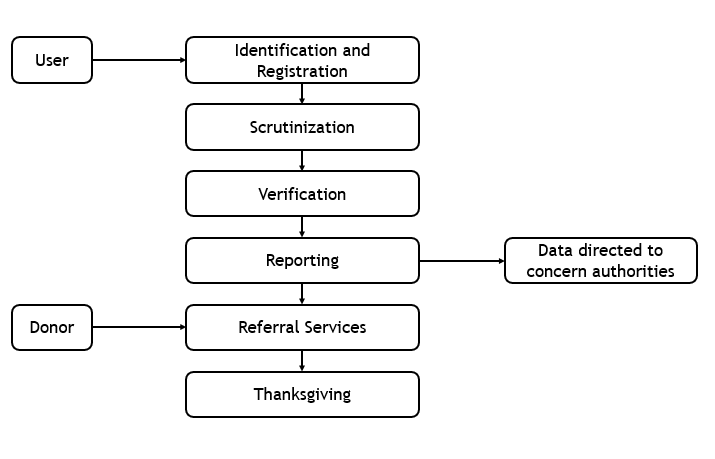
\includegraphics[width= 18cm,scale=0.70]{design/system arch.png}
    \caption{System Architecture }
    \label{fig:my_label}
  \end{figure}
    
    
    
    
\section{Data Flow Diagram}

 A data flow diagram (DFD) is a graphical representation of the ‘flow’ of data through an information system, modelling its process aspects. A DFD is often used as a preliminary step to create an overview of the system, which can later be elaborated. DFDs can also be used for the visualization of data processing (structured design). A DFD shows what kind of information will be input to and output from the system, where the data will come from and go to, and where the data will be stored.

\subsection{Level 0 DFD}
Level 0 contains one input and one output. The system provides information to the user means system is input and the user is output. Figure 4.2 shows Level 0 DFD of project.
\begin{figure}[H]
    \centering
    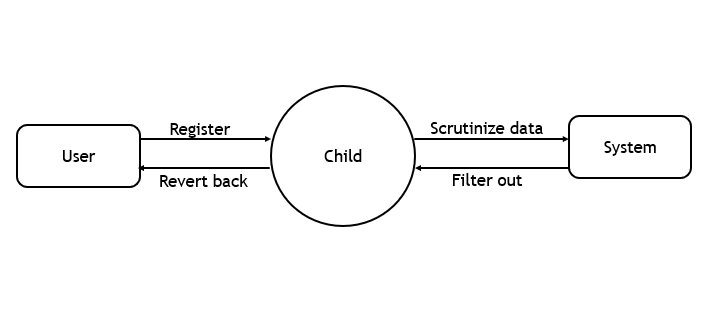
\includegraphics[width = 12cm]{design/0 level DFD.png}
    \caption{ 0 Level Data Flow Diagram}
    \label{fig:my_label}
\end{figure}

\subsection{Level 1 DFD}
A level 1 DFD notates each of the main sub-processes that together form the complete system.   We can think of a level 1 DFD as an “exploded view” of the context diagram. 
Figure 4.3 shows Level 1 DFD of project.
\begin{figure}[H]
    \centering
    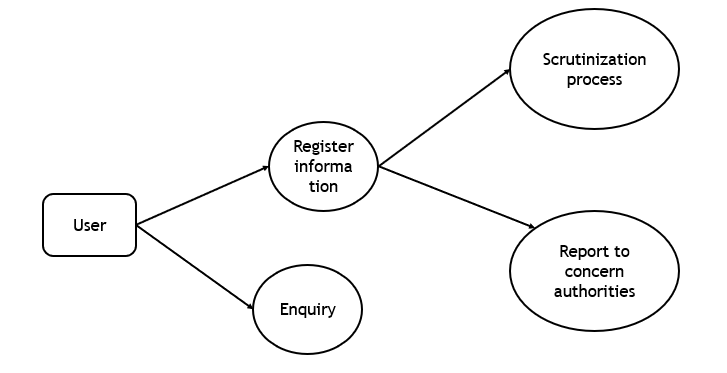
\includegraphics[width = 12cm]{design/1 Level DFD.png}
    \caption{  1 Level Data Flow Diagram }
    \label{fig:my_label}
\end{figure}


\subsection{Level 2 DFD}

A level 2 data flow diagram offers a more detailed look at the processes that make up an information system than a level 1 DFD does. It can be used to plan or record the specific makeup of a system.\\ Figure 4.4 shows Level 2 DFD of project.
\begin{figure}[H]
    \centering
    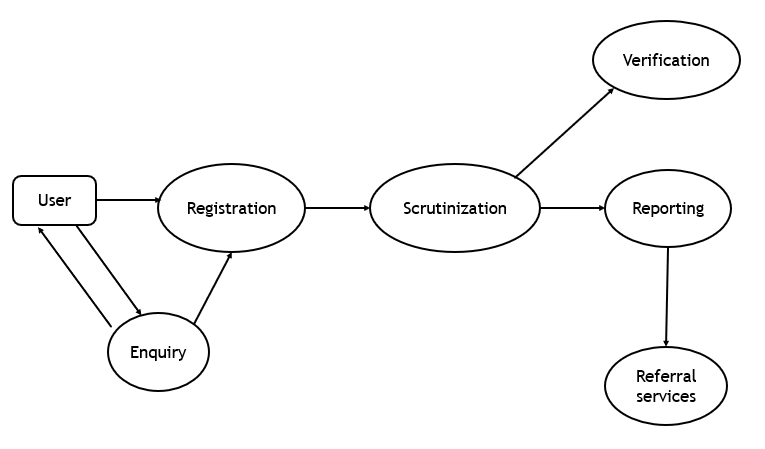
\includegraphics[width=12cm]{design/2 Level DFD.png}
    \caption{2 Level Data Flow Diagram}
    \label{fig:my_label}
\end{figure}

\newpage
\section{UML Diagrams}
A UML diagram is a diagram based on the UML (Unified Modeling Language) with the purpose of visually representing a system along with its main actors, roles, actions, artifacts or classes, in order to better understand, alter, maintain, or document information about the system.

\subsection{Use Case Diagram}
Use case diagram shows the interaction between Use case which represents system functionality and actor which represent the people or system. Fig 4.5 shows use case diagram.
\begin{figure}[H]
    \centering
    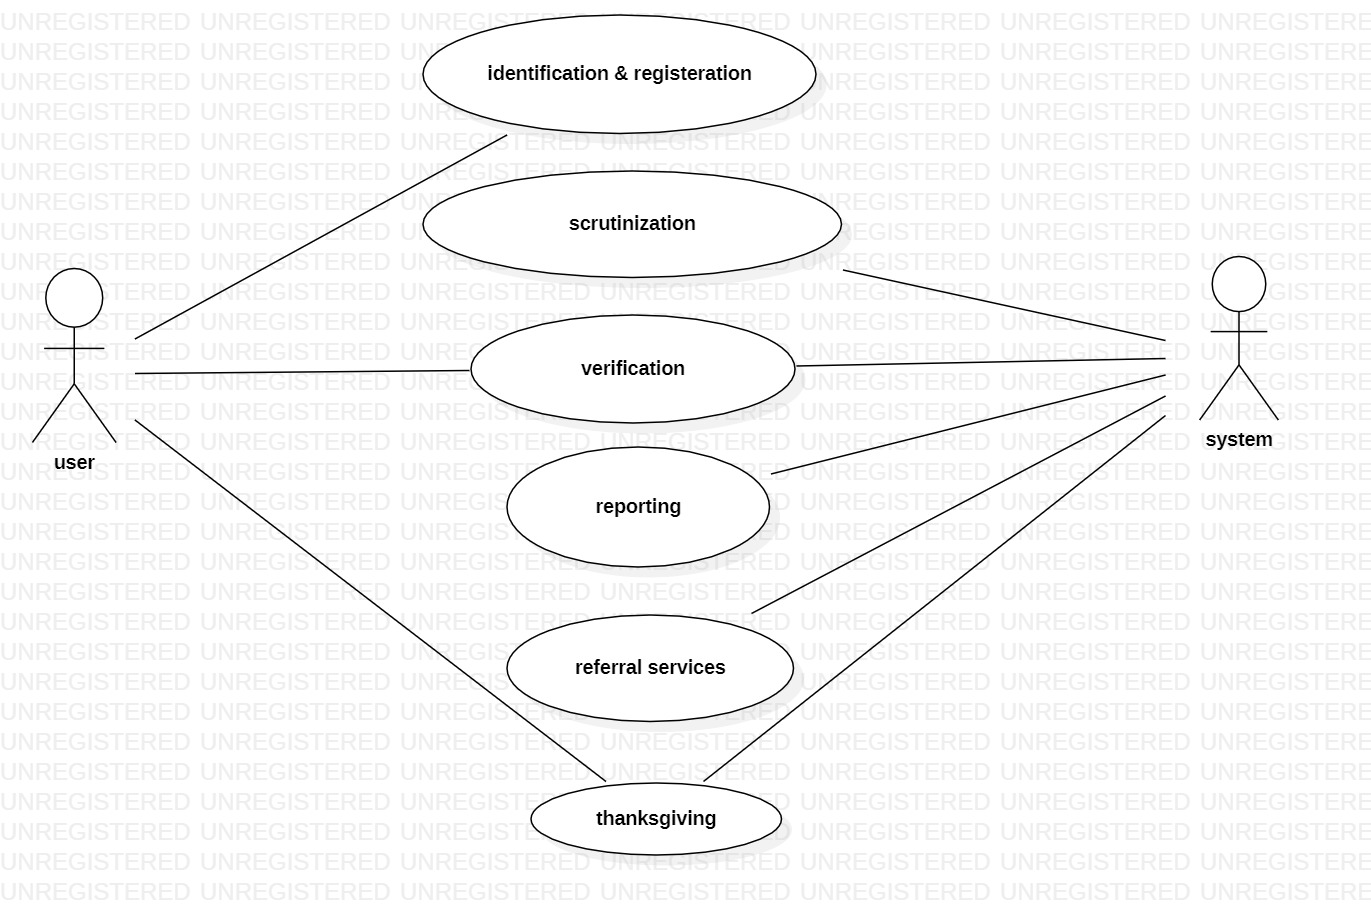
\includegraphics[scale=0.35]{design/usecase.jpg}
    \caption{Use Case Diagram}
    \label{fig:my_label}
\end{figure}


\subsection{Sequence Diagram}

The sequence diagram shows the flow of functionality through Use case. A sequence diagram is a type of interaction diagram because it describes how—and in what order—a group of objects works together. These diagrams are used by software developers and business professionals to understand requirements for a new system or to document an existing process.Fig 4.6 shows sequence diagram.

\begin{figure}[H]
    \centering
    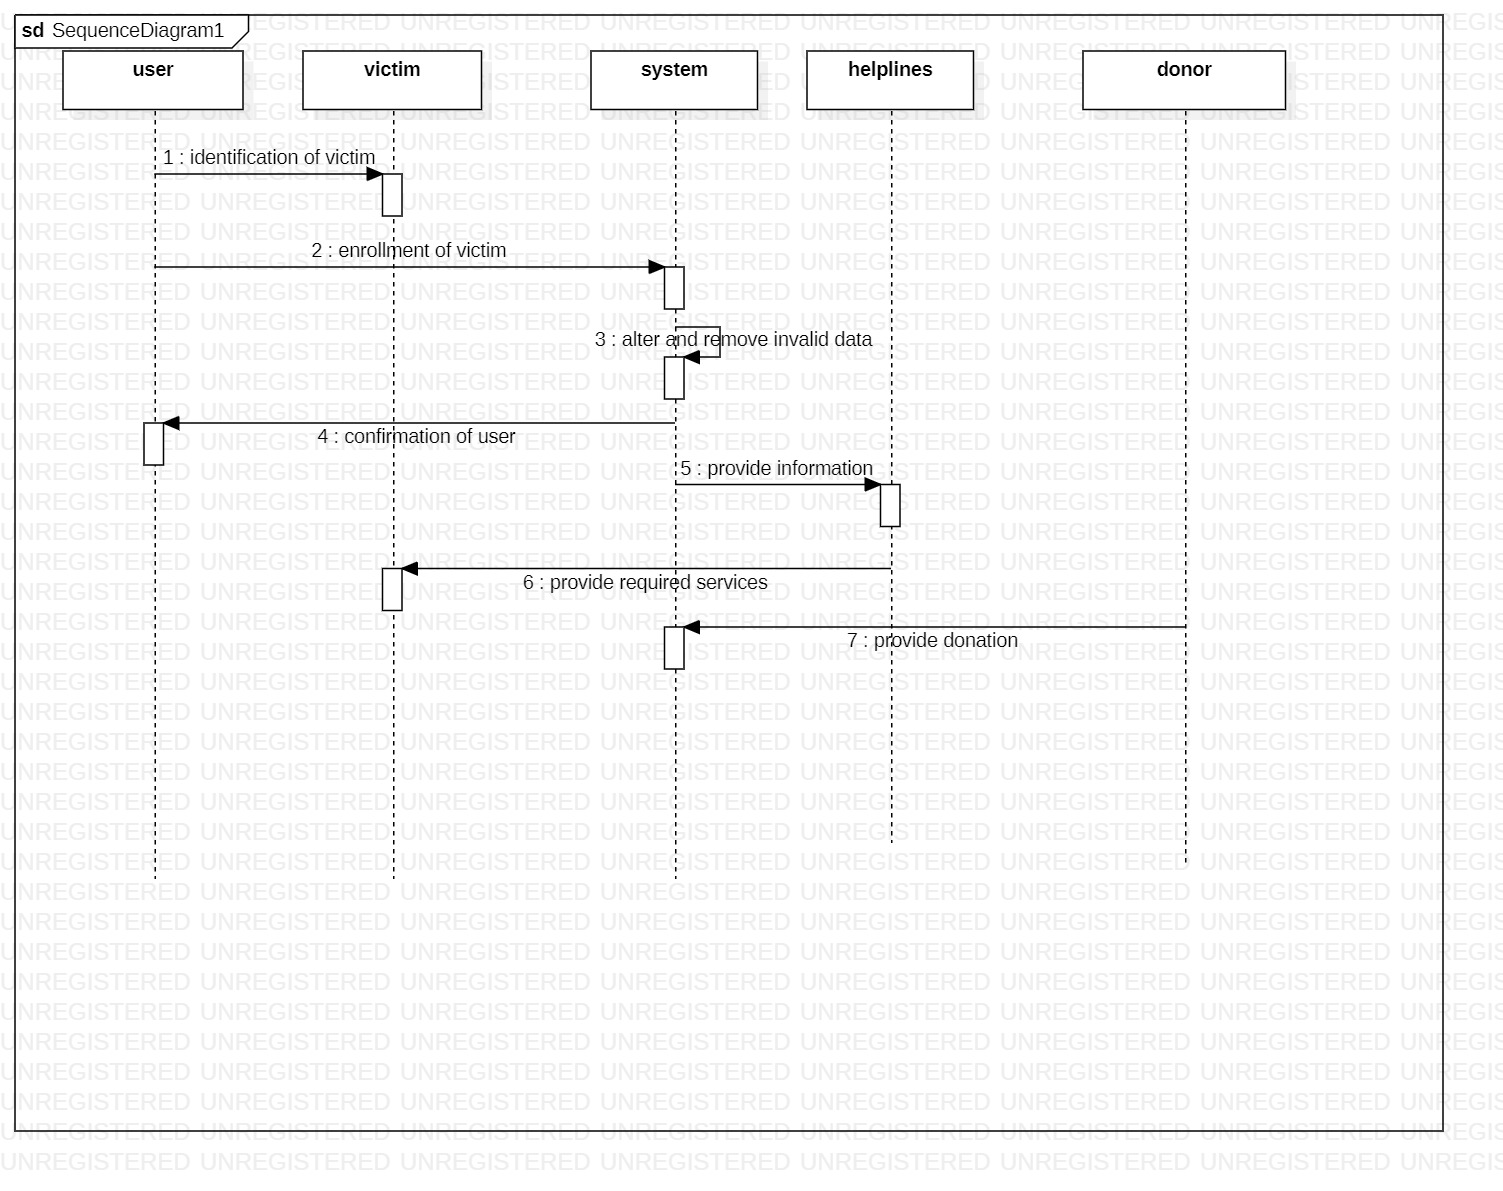
\includegraphics[scale=0.35]{design/SequenceDiagram.jpg}
    \caption{Sequence Diagram}
    \label{fig:my_label}
\end{figure}

\subsection{Collaboration Diagram}
A collaboration diagram, also known as a communication diagram, is an illustration of the relationships and interactions among software objects in the Unified Modeling Language (UML). These diagrams can be used to portray the dynamic behavior of a particular use case and define the role of each object. Fig 4.7 shows collaboration diagram.
\begin{figure}[H]
    \centering
    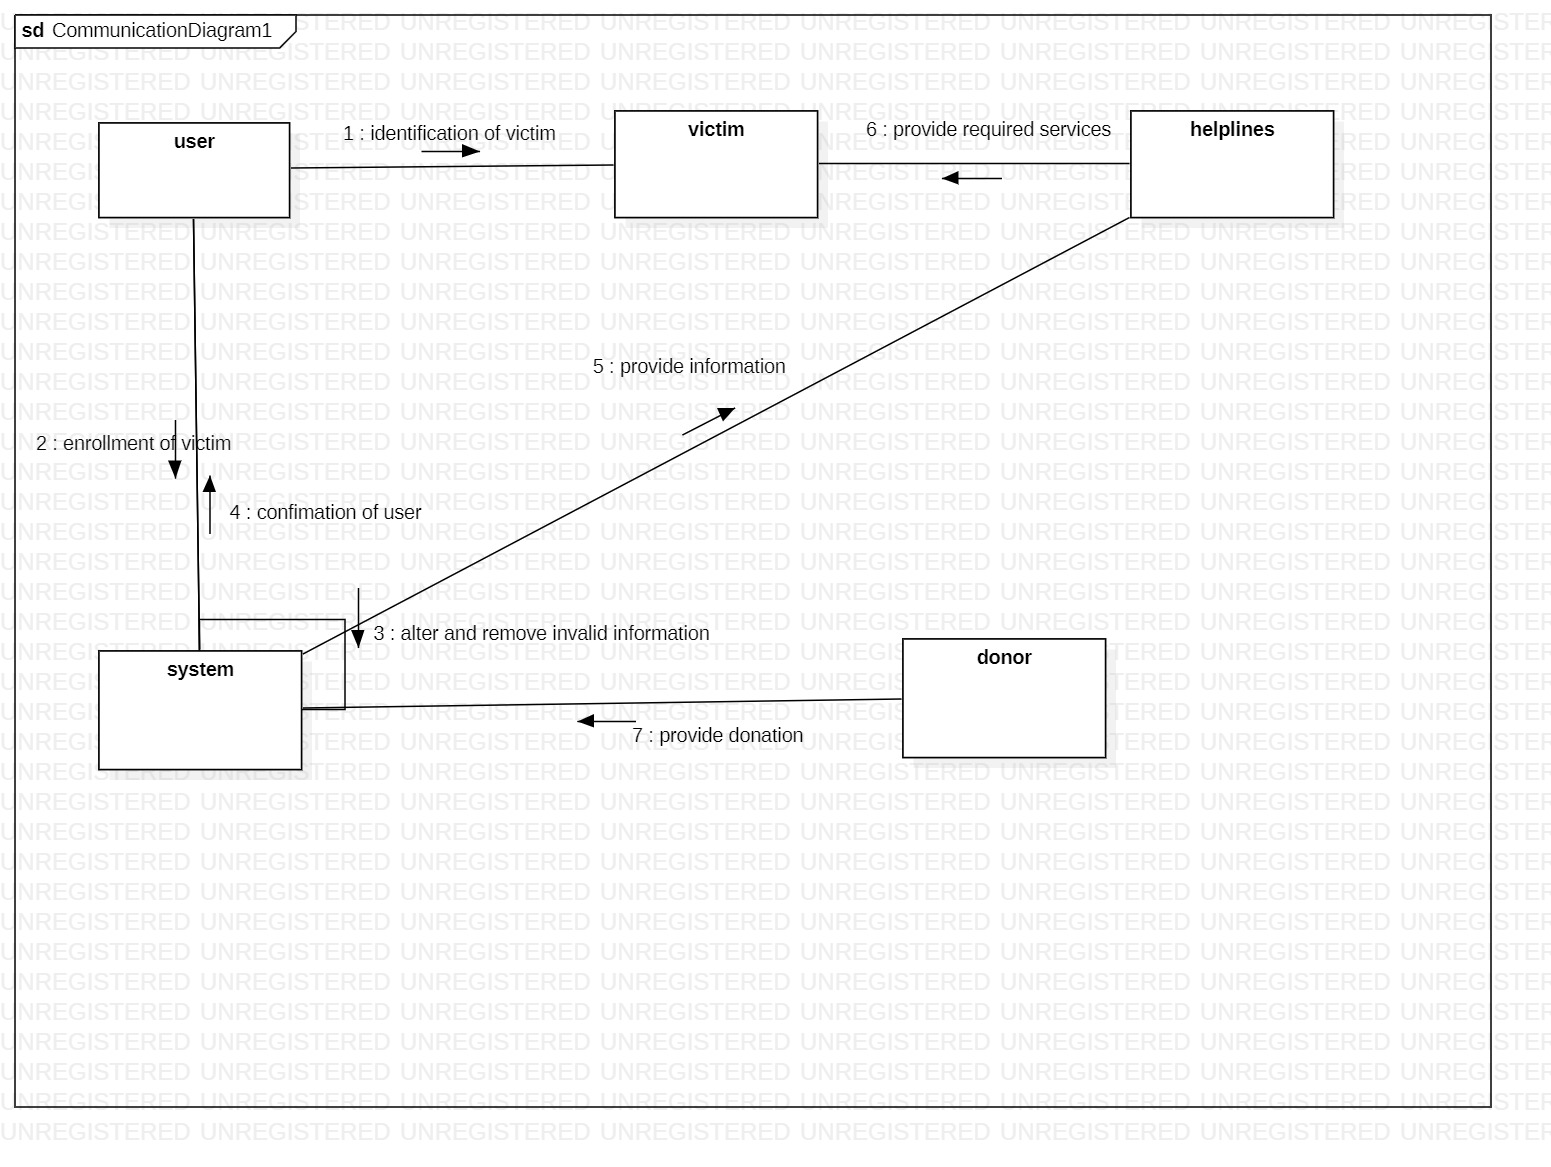
\includegraphics[scale=0.30]{design/CommunicationDiagram.jpg}
    \caption{Collaboration Diagram}
    \label{fig:my_label}
\end{figure}

\subsection{Class Diagram}
The class diagram is the main building block of object-oriented modeling. It is used for general conceptual modeling of the structure of the application, and for detailed modeling translating the models into programming code. Class diagrams can also be used for data modeling. Fig 4.8 shows class diagram.
\begin{figure}[H]
    \centering
    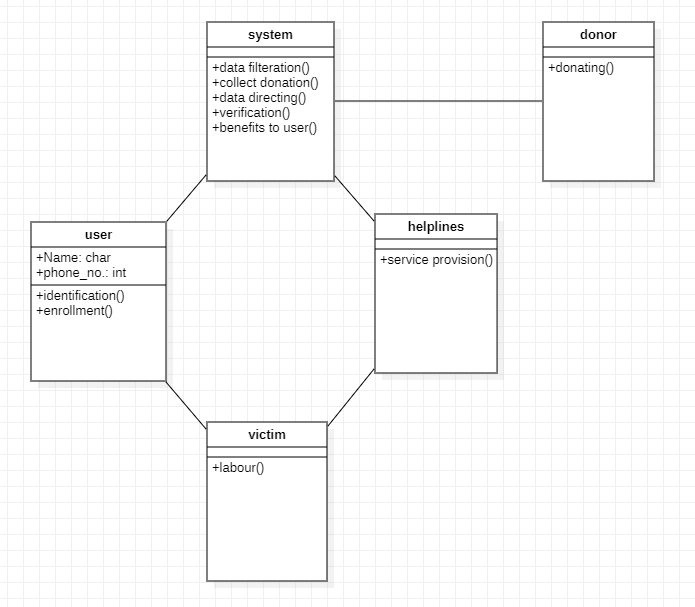
\includegraphics[scale=0.70]{design/ClassDiagram.png}
    \caption{Class Diagram}
    \label{fig:my_label}
\end{figure}

\subsection{Component Diagram}
A component diagram, also known as a UML component diagram, describes the organization and wiring of the physical components in a system. Component diagrams are often drawn to help model implementation details and double-check that every aspect of the system’s required function is covered by planned development.Fig 4.9 shows component diagram.
\begin{figure}[H]
    \centering
    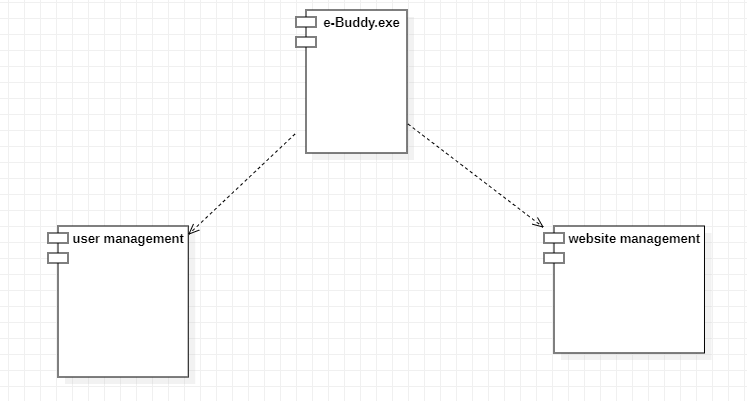
\includegraphics[scale=0.60]{design/ComponentDiagram.png}
    \caption{Component Diagram}
    \label{fig:my_label}
\end{figure}

\subsection{Deployment Diagram}
A deployment diagram is a UML diagram type that shows the execution architecture of a system, including nodes such as hardware or software execution environments, and the middle ware connecting them. Deployment diagrams are typically used to visualize the physical hardware and software of a system. Fig 4.10 shows deployment diagram.
\begin{figure}[H]
    \centering
    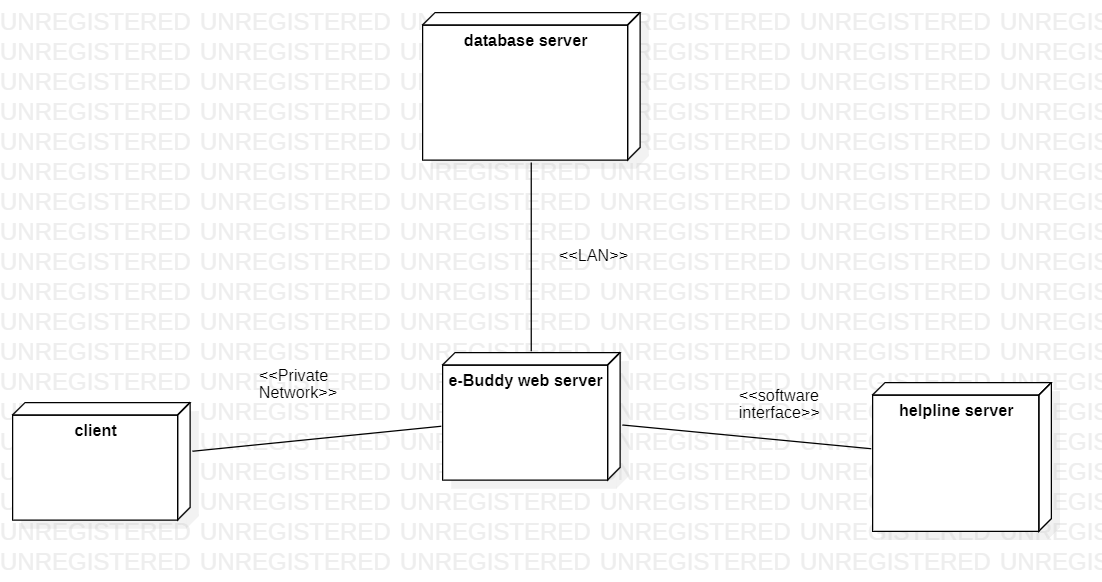
\includegraphics[scale=0.45]{design/DeploymentDiagram1.png}
    \caption{Deployment Diagram}
    \label{fig:my_label}
\end{figure}

\section{Summary}
Detailed design of project has been described in this chapter including the Data Flow Diagrams and the UML Diagram explaining all the design details of the project. Conclusion of the project has been explained in the next chapter. 